\documentclass[thesis.tex]{subfiles}

\begin{document}

\section{Overview} 
\epigraph{``Maybe the universe isn’t total chaos.''}{-- Annie Landsberg \\ Maniac, S1 E10: `Option C' (2018)}
% \Gls{latex} \gls{latex} \gls{lambda} $\theta = \gls{lambda}$ % LINDEN UNCOMMENT
Computational analysis of genomic data has transformed research and clinical practice throughout medicine. This effect has been especially strong in fields with a strong molecular biology component, such as oncology. While the generation of biological data has unlocked invaluable new resources, it has demanded complementary advancements in statistical and machine learning in order to answer theoretical and practical questions. The modern researcher has access to a catalogue of tools, including methods inspired by modern progress in AI from disciplines such as natural language processing and image analysis. However, before employing the latest and greatest technique 
from predictive or generative modelling, it is worth asking a sequence of questions. What sort of data are we dealing with in genomic medicine? Given the abundance of data available for a particular problem, what level of model complexity is appropriate? If our methods do work, will we understand why? What stage of the clinical pipeline is being targeted enough? If our hope is for the deployment of predictive systems in clinical settings, are our tools robust enough? If so, are the technologies upon which they rely economically viable? While we will certainly not answer all of these questions, in the chapters that follow we will provide some language with which to discuss them, and a range of application cases across genomic medicine. 

This introduction, which is adapted in part from the book chapter `Dimensionality and structure in cancer genomics: a statistical learning
perspective' \citep{bradley_dimensionality_2020}, should be equally approachable to those with a background in statistics/machine learning and those from biology. We'll begin with a contextualisation of genomics research as the starting point for much of modern medicine, including the discovery of diseases mechanisms, biomarkers, and therapeutics. We'll then discuss the role of predictive models in enabling `precision medicine', and their substantial challenges. In a complementary strand, we'll highlight the role of statistical learning theory in phrasing and interrogating biological questions, as well as serving as the backbone of modern developments in machine learning. After a brief introduction to the types of data encountered in sequencing-based studies and the opportunities and problems they present, we'll provide some terminology and useful concepts from high-dimensional statistics, Bayesian statistics, and causal inference, and will discuss how these concepts arise naturally in the context of genomic medicine. These will be accompanied by some illustrative examples of how different techniques may be employed in translational scientific research, but the bulk of description of specific applications is left to the following chapters. We will conclude with sketches of some modern developments, and a summary of the application cases considered throughout the rest of this thesis.

\subsection{Genomics in medicine}
Since the success of the Human Genome Project \citep{lander_initial_2001}, sequencing technologies
have improved at an exponential rate, both in terms of cost per megabase
sequenced \citep{wetterstrand_dna_2022} and the number of individuals who have had some portion of
their genome sequenced. Advances have also been made in sequencing accuracy and the capacity for long-read sequencing \citep{goldfeder_human_2017}. This has introduced an invaluable new resource
for biomedical research, and initiatives such as the 10,000/100,000 Genomes Projects \citep{telenti_deep_2016} and the UK Biobank \citep{bycroft_uk_2018} have drastically improved the accessibility and infrastructure surrounding this data \citep{szustakowski_advancing_2021}. This is beginning to show impact in clinical settings \citep{prokop_genome_2018}. In the study of cancer, a disease of the
genome, the ability to rapidly and cheaply sequence normal and tumour-derived \glsxtrshort{dna} has transformed basic research, birthing the field of cancer
genomics. While \glsxtrlong{wgs} is not yet standard of care for the generic cancer patient,
access to in-depth genetic data is becoming more common. Cancer-specific data repositories such as The Cancer Genome Atlas \citep{weinstein_cancer_2013} have given
researchers access to large clinical datasets with a variety of accompanying
genomics data. 

One use of genomic data in a clincal setting is for subtyping or endotyping patients in a way that informs treatment decisions -- a key tenet of so-called `personalised medicine' or `precision medicine'. This may involve categorisation in very broad terms, such as the separation of virally and bacterially infected patients (see Chapter~\ref{chap:lamp_modelling}; \citealp{remmel_diagnostic_2022}), or distinguishing tumours according to the molecular profile of their mutations \citep{zhao_molecular_2019}.

Understanding the genomic landscape of disease is also critical to the field of early-stage drug discovery \citep{nelson_support_2015, raja_integrating_2017, king_are_2019}. In cancer, knowledge of the location and associated products of oncogenes (genes in which mutation can cause a cell to become cancerous) can allow for intelligent selection of druggable sites \citep{weinstein_cancer_2002, bedard_small_2020}, and identification of tumour suppressor genes (genes which under normal circumstances prevent uncontrolled cell division) gives options for therapies which may replace cancer patients' defective cell cycle control mechanisms \citep{fang_tumor-suppressing_2003, morris_therapeutic_2015}. 

Alongside new drugs, it has become increasingly common for therapies to be offered alongisde genomic biomarkers which may stratify patients who are more likely to benefit from the treatment \citep{weber_egfr_2014, awad_precision_2019, zhu_association_2019, safarika_29-mrna_2021}. This is important for a variety of reasons: to prevent unnecessary suffering for patients unlikely to benefit from drugs with adverse side-effects; to minimise unnecessary cost of wasted treatments unlikely to succeed; and to allow management of the use of therapies for reasons such as anti-microbial stewardship.

New sources and types of data have allowed researchers a greatly expanded
toolbox with which to investigate the causes and development of cancer and to address the goals discussed above, but
also present a unique set of challenges. Firstly, in clinical settings it is commonly necessary (or at least very useful) to have some sense of the uncertainty accompanying any given prediction or assignment. Secondly, the number of covariates common in ’omics datasets induces a variety of theoretical and practical problems for classical statistical analysis, a problem often referred to as the curse of dimensionality \citep{barbour_precision_2019, buhlmann_high-dimensional_2014}. Finally, genomic datasets are often collected in observational settings, with limited interventional control, incomplete observation, and compiled from multiple heterogeneous data sources. In subsequent sections we introduce some of the methods developed to address each of these methodological challenges.

\subsection{Statistical learning and machine learning} 
Informally, the fields of statistical learning and machine learning attempt to address the
theoretical and computational challenges associated with extracting information from data. In each case, the use of the word `learning' is commonly taken to imply some future reuse of the information extracted by the fitted (or `trained') models. Often, this reuse comes via re-applying a fitted model to a given prediction task, e.g. a regression or classification. The distinction between machine learning and statistical learning is vague and constantly evolving. Broadly speaking, the following trends are informative but not prescriptive in describing statistical vs machine learning: \emph{1)} an emphasis in statistical learning on theoretical and mathematical guarantees on the future performance of predictive models; \emph{2)} a tendency towards scale and non-linearity as a features of machine learning models; \emph{3)} recently, a specific focus in machine learning on neural networks and deep learning; and \emph{4)} in machine learning, a greater attention to and study of the deployment of models, including software development and operations (spawning the field of MLOps), model drift over time, and interaction with hardware during both training and prediction. 


\jbnote{Open debate around the role of structure in NLP and IR. Remains to be seen what'll work in bio} Recent decades have seen much excitement around the application of machine learning methods to a wide variety of high-dimensional problems. Particular progress has been made in automated image recognition and natural language processing (NLP). This progress has come via the development of specialised techniques to exploit the \textbf{structure} inherent in each data type (for example convolutional neural networks for image recognition \citep{liu_review_2017} and word embedding for NLP \citep{gutierrez_systematic_2019}, but also from a vastly increased pool of data on which to train models. These data resources have typically been collected online, where there exists an abundance of labelled and unlabelled images and pieces of text. 

It is hoped that similar strides forward can be anticipated in biology, but it is important to acknowledge the current gap in data availability between cancer genomics and the other machine learning disciplines mentioned above. In the next section we will discuss typical types of biological data encountered in cancer genomics (including sequencing-based genomics technologics that may not strictly be genomics, such as gene expression profiling), their dimensionality and typical availability. While efforts to deploy machine learning architectures are certainly producing results in some cases \citep{dubourg-felonneau_flatsomatic_2019, dubourg-felonneau_learning_2019}, an important takeaway is that in many cases, we are not yet in a situation where the data-heavy deep learning approaches that have revolutionised image recognition will be applicable to cancer genomics problems. 

That is not to say that we can't do anything! In fact, it is often instructive to try and make headway in situations where a `data-heavy, structure-light' approach is unsuitable, and these sorts of investigations can have a profound impact on the design of more sophisticated models \citep{buhlmann_high-dimensional_2014}. As a final point, readers approaching without a significant backlog of machine learning expertise will find that an understanding of statistical terminology will aid comprehension of the machine learning literature which has them as its basis.

\section{Genomics and biological data}
\epigraph{``En particulier, on ne
saurait préciser actuellement le mécanisme selon lequel
les gènes désoxyribonucléiques peuvent commander l'édification des acides ribonucléiques cytoplasmiques et le
mécanisme selon lequel ces acides ribonucléiques
peuvent présider à l'élaboration des enzymes...''}{\citet{boivin_sur_1947}}

In this section we'll briefly review some of of the central tenets of molecular biology as they apply to the rest of this work. In particular, we'll focus on how information flows between the three classes of molecule whose interactions determine the majority of cellular functionality. These are \glsxtrshort{dna}, \glsxtrshort{rna}, and proteins, and the flow of information between them is so consistent across nature that it is referred to as the `central dogma' of molecular biology. Describing this process also allows us to exhibit the main new sources of data that have enabled the genomics (alternately just `omics', to distinguish from \glsxtrshort{dna}-only analysis) revolution, and to give context to their respective uses and limitations. 

Once we've reviewed the (thankfully very little) molecular biology necessary for subsequent chapters, we'll discuss the specific role of genomics data in medicine and the study of disease. Because cancer forms the dominant thread of the second half of this thesis (and because it's so incredibly interesting), we'll devote extra time to discuss some fundamental concepts from cancer genomics. We'll then go into more detail in the specifics of modern technologies for sequencing and quantification across major genomics data types.

\subsection{The central dogma}
Molecular biology, historically, has enabled the successful collision of two major subfields of biology. On the one hand, evolutionary biology has concerned the role of inheritance and diversity in producing the range of organisms observed in the natural world. On the other, cellular biology has concerned the mechanistic operation of cells, the constituent units of all living beings. Molecular biology provides the link between these two disparate areas of study via the flow of information between two classes of molecule. Firstly, \gls{dna} is the carrier of genetic information and provides the mechanism for Mendelian and Darwinian inheritance. Secondly, proteins are the machines that, at the lowest level of resolution, perform the tasks that sustain and manage the operation of cells in sickness and in health. We now have a fairly nuanced understand of the connections between the two, with \gls{rna} sat between them in the role of `messenger'\footnote{In reality, \glsxtrshort{rna} does a lot more than just this. As far as the central dogma goes, however, this is \glsxtrshort{rna}'s main function.}. Molecular biology, via a number of key results including the discovery of the structure of \glsxtrshort{dna} in the 1950s by Crick, Franklin, Watson and Wilkins \citep{franklin_molecular_1953, watson_molecular_1953, wilkins_molecular_1953, maddox_double_2003}, the role of \glsxtrshort{rna} as an intermediary between \glsxtrshort{dna} and proteins \citep{boivin_sur_1947, crick_protein_1958, brenner_unstable_1961, cobb_who_2015}, and the `cracking' of the genetic code \citep{crick_general_1961, nirenberg_rna_1964, brenner_uga_1967, tamura_genetic_2016}, enabled a conceptual and practical bridge
between disciplines and a fundamental unification of modern biology. 

The central dogma, a term coined by Crick, can be described as follows (see also Figure~\ref{fig:central_dogma}). Contained within the nucleotide sequence of \glsxtrshort{dna} -- often represented as a string of letters $A$, $C$, $G$ and $T$,  representing the nucleotide bases adenine, cytosine, guanine and thymine respectively -- is the hereditary information of an organism. As is necessary for replication at the cell or organismal level, \glsxtrshort{dna} can be copied with the help of an enzyme known as a \glsxtrshort{dna} polymerase. This is represented by a cyclic arrow from \glsxtrshort{dna} to itself in Figure~\ref{fig:central_dogma}. With the aid of an enzyme known as an \glsxtrshort{rna} polymerase, \gls{mrna} molecules can be can be `transcribed' from a \glsxtrshort{dna} sequence. This leaves the \glsxtrshort{dna} molecule unchanged in its nucleotide information content but produces a single-stranded \gls{mrna} molecule that may be transported out of the cell nucleus where \glsxtrshort{dna} is typically stored. The word `transcription' is used to emphasis that, while chemically slightly different, \glsxtrshort{dna} and \glsxtrshort{rna} are essentially expressing the same language, with the nucleotides $A$/$C$/$G$/$T$ in \glsxtrshort{dna} directly mapping to the nucleotides $A$/$C$/$G$/$U$ in \glsxtrshort{rna} (the letter U in represents the nucleotide uracil, itself only differing from thymine by a single methyl group). Like \glsxtrshort{dna}, \glsxtrshort{rna} may also be used as a template for direct replication with the aid of an \glsxtrshort{rna} replicase enzyme, also known as \gls{rdrp}.

\begin{figure}[htbp]
\centering
\begin{tikzcd}[row sep = small, column sep = large]
DNA \arrow[loop above] \arrow[r, "transciption"] & RNA \arrow[loop above] \arrow[r, "translation"]  \arrow[l, bend left, dashed, "reverse \ transcription"] & Protein \\
& & \\
(Data) & (Message) & (Action) 
\end{tikzcd}
\caption{The central dogma.\label{fig:central_dogma}}
\end{figure}

For a typical gene, \glsxtrshort{rna} molecules are transported to the cytoplasm of the cell and, in structures known as ribosomes -- themselves built out of a mixture of \gls{rrna} and protein -- are \emph{translated} to proteins. Proteins are composed of sequences of amino acids, of which there are twenty. Each amino acid is associated with a set of three-nucleotide \emph{codons}, with special codons also associated with starting and stopping translation. Together, this collection of codon-to -protein-instruction maps are referred to as the `genetic code'.

The central dogma refers to the one-directional flow of information along the \glsxtrshort{dna} $\rightarrow$ \gls{mrna} $\rightarrow$ Protein chain. Crucially, while genetic information contained in nucleic acids can be converted to protein via translation of \gls{mrna}, the reverse will never occur. It was historically unclear whether the one-directional flow of information would extend to transcription of \glsxtrshort{dna} to \glsxtrshort{rna}. This was settled when it was discovered that the conversion of \glsxtrshort{rna}  to \glsxtrshort{dna}  via reverse transcription, while rare in nature, is demonstrated by various retroviruses \citep{baltimore_rna-dependent_1970, temin_rna-dependent_1970, coffin_discovery_2016}. Nowadays, reverse transcriptiontechnology  is commonly used throughout genomic research, for example as part of sample preparation for the clinical gene expression testing approach described in Chapter~\ref{chap:lamp_modelling}. This test also makes extensive use of \glsxtrshort{dna} polymerisation at each reaction stage.

The three classes of molecule described by the central dogma are also the basis of the main new data sources that have powered the genomics revolution of the last two decades.

{\color{red}
\begin{enumerate}
    \item Sanger sequencing
    \item Gene expression, translation and biological function
    \item northern blots and western blots?
    \item genomics, transciptomics, proteomics, everything 'omics
\end{enumerate}
}

\subsection{Genomics in disease}
{\color{red}
\begin{enumerate}
    \item Discovery of inherited diseases
    \item Identification of disease-causing genes
    \item Polygenic risk scores
    \item Treatments designed to suppress genes
    \item Treatments design to replace genes 
    \item Accompanying genomic biomarkers
\end{enumerate}
}
\subsubsection{Cancer: a disease of the genome}
Cancer does not require much introduction even to the lay reader; direct or indirect experience of cancer is universal. It is consistently ranked amongst the leading causes of global mortality, and multiple subtypes of cancer are projected to increase in their ranking and share of worldwide premature deaths over the coming decades \citep{mathers_projections_2006}, including in the developing world \citep{kanavos_rising_2006}. Beyond its direct death toll, cancer is responsible for the expenditure of trillions of dollars per year in cost of care and lost economic output \citep{wild_world_2020}. While huge gains in the understanding, prevention and treatment of cancer have been made in recent years, many challenges remains in scalably advancing each of these areas. Modern cancer treatments in particular are often extremely expensive, with drug development costs increasing and consequently inflating the price of access to therapeutics \citep{howard_pricing_2015}. In short, there is much to be hopeful about in oncology, but it is by no means guaranteed that the current revolutions being enjoyed in scientific understanding will translate fully to equitable clinical benefit.

In order to understand the state of play in cancer research, we need to know a little about the nature of cancer itself, and in particular about cancer genomics beyond the general introduction to molecular biology given above. A key starting point is that cancer is not a unitary disease;  two patients’ tumours may be caused by different processes, occur in different tissues, and have very different molecular and physiological effects \citep{wittekind_tnm_2016}. More so than any other disease, every cancer and every tumour are unique. It is therefore natural to ask what unifying features of all cancers justify their joint classification. The modern answer is distinct from the historical answer. Before the advent of molecular genetics, cancers of disparate tissues of origin were grouped together because of the common observation of malignant growths crossing over physiological boundaries. Towards the end of the 19th century, it was recognised that aberrant patterns of cell reproduction were a common feature of cancers \citep{weinstein_history_2008}. By the early 1900s, with the writings of scientists such as Theodor Boveri \citep[see][for a modern translation]{boveri_concerning_2008}, an answer would be formulated foreshadowing our current understanding, although it wouldn't be until far later that this explanation was fully accepted. Boveri proposed that `chromosomal abnormalities' gave rise to the conversion of normal cells to malignant neoplasms. In modern nomenclature, the chromosomal abnormalities to which he referred would be regarded as (a specific kind of) mutations. It is these that lay the groundwork for uncontrolled cellular reproduction and all the other associated hallmarks of cancer\footnote{While some rare cancers such as \gls{pv} may involve uncontrolled production of cells that do not themselves harbour mutations (in this case, mature red blood cells do not contain \glsxtrshort{dna} at all), this is still the downstream effect of mutations in other cell types. For example, in \gls{pv} this is most commonly a mutation of the \textit{JAK2} gene in hematopoietic stem cells \citep{tefferi_jak2_2007}.}, such as avoiding detection from the body's defenses (immunosuppression/evasion), recruiting a local blood supply (angiogenesis), and invasion of separate tissues (metastasis) \citep{hanahan_hallmarks_2011}. Crucially, mutations convert previously normal or benign cell populations into tumours. The mutations that were observable via optical microscopy to scientists in the first half of the twentieth century were structural mutations involving large-scale chromosomal translocations or deletions. It wasn't until the identification of the structure of \glsxtrshort{dna} and its role as the primary mechanism of inheritance by Franklin, \citet{watson_molecular_1953} and the subsequent development of molecular genetics that the discrete nature of biological information was fully appreciated. Later developments in \glsxtrshort{dna} sequencing, beginning with the work of \citet{sanger_dna_1977} allowed a fuller understanding of mutations as changes to the sequence of nucleotide bases that constitutes \glsxtrshort{dna}. The science of cancer continued to progress by associating \glsxtrshort{dna} mutations (errors of cellular information storage), with their mechanistic and functional consequences, in particular those that led to deregulation of normal cell-cycle control.

Now that we are armed with a general characterisation of cancer as the consequences of mutations in \glsxtrshort{dna} leading to abnormal reproduction of cells, we can begin to appreciate the reasons for cancer's diversity. Since almost all cells in the body contain \glsxtrshort{dna} and experience regular reproduction, cancer may occur in a wide range of tissues throughout the body\footnote{Note that tissues/cell types in which cancer is extremely uncommon tend to be those which experience very little reproduction, and so have little chance to accumulate mutations, e.g. neuronal cells and tissues making up the heart.}. Furthermore, the size of the human genome (defined as the combined total of genetic information contained in \glsxtrshort{dna}, comprising of around 20,000 genes and 3 billion nucleotide base pairs) means that, even with cancer being as common a disease as it is, simple statistical reasoning allows us to say with confidence that it is almost inconceivable that two given tumours would carry exactly the same constituent mutations (even without considering complicating factors such as tumour heterogeneity). This leads us to the modern era of molecular biology. Since the completion of the human genome project \citep{lander_initial_2001}, high-throughput sequencing, where large portions of the genome in their entirety are sequenced for a biological sample, has become ubiquitous and highly automated. We now have easy access to the precise locations of all mutations in the tumour genomes of many tens thousands of thousands of samples gathered across hundreds of studies via repositories such as \gls{tcga} \citep{weinstein_cancer_2013}. This gives us an opportunity to investigate a variety of fundamental questions with regards to the progression of cancer. One of these mirrors a classic debate of nature versus nurture in developmental biology. In this case, we wish to understand the extent to which the dynamics and trajectory of a tumour are pre-determined by the genetic damage it carries. We know that cancers are defined by their mutations, but a growing field of investigation is exploring the role of the environment in which a tumour finds itself in allowing it to flourish. For the remainder of this section, we will elaborate on the balance between these two views of the tumour genome.

\subsubsection{Nature vs nurture: cancer beyond the genome}

\subsection{Modern sequencing technologies}
Cancer genomics is underpinned by the ability to sequence \glsxtrshort{dna} cheaply and quickly. \glsxtrshort{dna} is organised into chromosomes, along each of which many genes are arranged, with further non-coding regions interspersed in-between. The fundamental units of \glsxtrshort{dna} are nucleotide bases, of which there are four varieties (labelled C, G, T and A). These are organised in groups of length three called codons, which code for the production amino acids. Codons are arranged in sequences such that their amino acids when joined in chain form proteins - the products of genes. 

The aim of sequencing is to read, base by base, the information content of \glsxtrshort{dna}. This was originally done by Sanger sequencing, a procedure to infer the base composition of a piece of \glsxtrshort{dna} one base at a time. High-throughput sequencing automates this process via the following workflow:
\begin{enumerate}
    \item \glsxtrshort{dna} is isolated from a sample and amplified (replicated many times) to ensure good signal.
    \item Purified \glsxtrshort{dna} is broken into many pieces of manageable length.
    \item These short strands are sequenced individually and simultaneously by an automated process similar to Sanger sequencing.
    \item These short sequences are matched to a reference human genome to identify where the \glsxtrshort{dna} in the original sample differed from that reference.
\end{enumerate}

\subsubsection{Tumour/normal variants}
In cancer, some subset of cells accumulate mutations, via random misreplication of \glsxtrshort{dna} during cell division or exposure to some external mutagen (e.g. cigarette smoke, \gls{uv} light). Tumour cells therefore contain \glsxtrshort{dna} with a different sequence to that of the patients' typical sequence. To understand this two samples are collected, one from the tumour and one from normal tissue, and both are sequenced. The sequences are compared and this produces a list of locations at which mutations have occured: these mutations can have a variety of types (replacements, insertions, etc.) and can have vastly differing functional implications.

In simplest setting, we could express a tumour's mutational profile as a vector, with each component corresponding to whether the tumour-derived and normal sequences match at that point. How long would this vector be? The human genome contains approximately $3\times 10^9$ base locations. This is the dimensionality (which we'll refer to later on as $p$) of naively presented genomic data. We often like to compare the dimensionality of a dataset with the number of samples (which we'll later call $n$) to which we can expect to have access. In this case, unless we have access to tumour profiling for more than a third of all humans on the planet, we can never hope that these numbers will be comparable. We could make a small gain by listing all codons in the genome, labelling a component as one if the codon has been functionally altered by mutations and zero otherwise. Here though we would still have $p = 10^9$.

We could simplify our data further. Decades of biological research has focused on cataloguing the locations of genes across the genome. We might consider as covariates each of the (approximately $2\times 10^4$) genes, and represent each sample as a vector where each component refers to \textit{a)} whether or not the gene contained a functional mutation, \textit{b)} how many such mutations were present, or \textit{c)} some other representation of the severity of collective mutations presents in the gene, drawing upon known biology. It's important to appreciate the trade-off we've made here: we've imposed an external notion of structure onto our data and in return have greatly reduced the dimensionality (by five orders of magnitude), but in exchange have lost resolution and thus potential information. This gain/sacrifice will be reflected when we choose to make even further structural assumptions in order to construct sensible models.

\subsubsection{Heterogeneity and depth}
Another important concern for those dealing with cancer genome data is that tumours are often highly heterogeneous. Different sub-populations of cells have different mutation profiles, which fit into an evolutionary hierarchy within the tumour's history. The importance of understanding the role of heterogeneity is beginning to be appreciated in a clinical context, and this has implications for the type of data that are used. In the context of the high-throughput sequencing pipeline, the relevant quantity is depth: identifying not just one but a variety of tumour sequences at a genomic locus along with the proportion in which they occur means thinking very hard about how best to express that data.


\subsection{Gene expression}
It is often not just the sequence of a gene which it relevant in a tumour, but the level of gene expression. The way that this is most often estimated is via the proxy of \glsxtrshort{rna}  transcript abundance: \glsxtrshort{rna}  is a similar molecule to \glsxtrshort{dna} that is produced during the process of \glsxtrshort{dna} being 'read', and acts as a messenger for sequences that should be converted to protein. Abundances of different \glsxtrshort{rna}  transcripts can be measured using procedures based on \glsxtrshort{dna} sequencing. This will in general give data with the same dimensionality as gene-based mutation data, but is of a different type. Measured values are continuous to represent concentrations of gene products, rather than discrete 'mutated/not mutated' values. This has implications as to the sort of structural assumptions we can make about the data that we observe, and the models that will be best suited to capitalise on that structure.


\section{Statistical learning theory}
\epigraph{``We need data to construct prediction rules, often a lot of it.'' \\
~\\
``For prediction purposes, [linear models] can sometimes outperform fancier
nonlinear models, especially in situations with small numbers of training
cases, low signal-to-noise ratio or sparse data.''}{Elements of Statistical Learning \\
\citep{hastie_elements_2009}}

Now familiar with the most relevant biological concepts, we turn to the mathematical theory and techniques underlying statistical learning, which has experienced a surge of interest in the last few decades, partially fuelled by explosions of data availability across multiple domains, contemporaneous increases in computational power, and the desire to provide satisfying theoretical frameworks to accompany complementary practical advances in machine learning. While so far there is certainly no theory of statistical learning with the capacity to fully describe, explain, or validate the impressive results demonstrated in (for example) deep learning, the language of statistical learning is invaluable in specifying learning models, providing metrics by which they can be measured, and triaging where they go wrong. It is also the language with which we will be attempting to interrogate issues of inference and prediction in cancer genomics. 

First some terminology and notation. In the work described here, we'll principally be concerned with \emph{prediction} settings\footnote{We consider this as not exactly equivalent to `supervised' settings. To us, prediction $\Leftrightarrow$ a downstream task involving predicting an outcome from inputs, whereas supervised $\Leftrightarrow$ all training data is formed of input/output pairs. So semi-supervised learning is not strictly supervised but may be a prediction task, whereas \gls{ols} for inference only is supervised but not a prediction task.}. We often consider a very generic setup, in which we have paired data
\[\mathcal{D}_n = \{(x_1, y_1), (x_2, y_2), \dots, (x_n, y_n)\}.\] 
We refer to this dataset as our `training' data. For full flexibility, we allow for the possibility that some response values $y_i \ (1 \leq i \leq n)$ may be missing. We do not consider settings in which inputs $x_i$ or any of their components are missing. We model each of these pairs as being drawn from a joint probability distribution $P_{X \times Y}$ which gives the probability of observing any combination of observation $x$ and label $y$. For now we make no assumptions about the nature of the $y_i$ labels: they may be continuous values (regression), discrete values (classification), or more complicated hybrid objects such as is the case in survival analysis (see Sections~\ref{sec:intro_survival}~and~\ref{sec:survival}). We assume that $x_i \in \mathbb{R}^p$ for each $1 \leq i \leq n$, so that our observed values are vectors of length $p$ and each element is a real number (possibly restricted to some subset such as the positive reals - this is what $\mathcal{X}$ specifies). We refer to $p$ as the dimension and $n$ as the sample size of our data. We wish to fit some model $\mathcal{M}$ to the data. This could be in order to make some inference about the parameters of the distribution $P_{X \times Y}$ which will hopefully shed light on the effect of each of the covariates contained in an observation $x$. Alternatively, we might be trying to predict future values of $y$ from unlabelled observations as accurately as possible. These two aims are often distinguished by the umbrella terms statistical inference and statistical learning.


\subsection{Bayesian and frequentist approaches to statistical inference and prediction}

\subsection{High-dimensional statistics}
% In these settings results such as the central limit theorem which rely on divergence of the sample size independent of the dimensionality are often not of much use \citep{wainwright_high-dimensional_2019}. This is often the case in cancer genomics. 

Informally, we may think of high-dimensional statistics to be concerned with the realm in which the dimensionality of our input data, $p$, is comparable to or greater than the number of training samples $n$ we have available. In this regime the classical asymptotic theory of statistics, which generally relies on an assumption of fixed dimension and considers limiting behaviour as $n \rightarrow \infty$, may fail to apply. Classical results such as the law of large numbers and central limit theorem are not applicable. 

In many statistical models we have a vector $\mathbf{\beta}$ of parameters with at least the same dimension as our data ($\mathbf{\beta} \in \mathbb{R}^q, \ q \geq p$). In generalised linear models (GLMs) the likelihood of an observation $y$ depends upon the data $x_i$ solely via the inner product $x_i^T\mathbf{\beta}$, so that each component of $\beta$ corresponds to the relative importance of its associated covariate. Classically, we would attempt to to estimate the parameter $\beta$ via our observation through a procedure such as likelihood maximisation. However, it is clear in this context that if $p$ is comparable to or larger than $n$ then we have very little chance of accurately inferring the parameter vector $\beta$. For example, we can't expect to simultaneously learn about the effect of 20 covariates if we only have 10 observations: we say here that the model is unidentifiable. 

High-dimensional statistics attempts to gauge what we can do in regimes such as these. One is approach is to assume the data has some low-dimensional structure. This means that we can embed our data in a lower dimensional space such that the smaller representation of our data contains all or most of the necessary information about the joint distribution $P_{X\times Y}$. We will discuss some common structural assumptions. The simplest and most interpretable is sparsity. \\~\\

\hrule 
\begin{definition}{\textbf{(Sparsity) "Relatively few covariates are important"} \label{def:sparse}} \\
Given a vector $\beta \in \mathbb{R}^p$ parameterising a model, we say $\mathbf{\beta}$ is $k$-sparse, for $k \leq p$, if at most $k$ elements of $\mathbf{\beta}$ are non-zero, i.e.
$$|\mathbf{\beta}|_0 := \sum_{j=1}^{p}\mathbbm{1}\{\beta_j \neq 0\} \leq k. $$
We can say a model $\mathcal{M}$ parameterised by a vector $\beta$ is $k$-sparse if the vector $\beta$ is $k$-sparse.
\end{definition}
\hrule 
~\\~\\

Sparsity is a useful assumption to make for a variety of reasons. We are reducing the number of parameters that we must estimate- for a $k$-sparse model, we need only estimate $k$ parameters. Before we do so we need to decide which $k$ parameters are allowed to be non-zero, i.e. to which $k$-dimensional subspace (out of $\begin{pmatrix} p \\ k \end{pmatrix}$ choices) our parameter belongs. In practice this is not a huge issue - some powerful theory from the field of convex optimisation allows for efficient training of sparse models (see the LASSO estimator below). Finally, sparse models are interpretable. A small number of covariates selected for importance can be useful in hypothesis refinement.

\subsubsection{Sparse data vs sparse models}
It is worth at this point drawing a distinction between two phenomena in statistics and data science both referred to as 'sparsity', both of which are exhibited in cancer genomics. The first is sparse \textit{data}, in which almost all observed data points have the same value (typically zero). Mutation data displays this trait- the rate at which mutations occur in the genome varies widely across and within cancer types, but rarely exceeds 100 Mut/Mb, i.e. one mutation per $10^4$ nucleotide base pairs \citep{chalmers_analysis_2017}. This sparsity is exploited in the way that tumour/normal \glsxtrshort{dna} data is stored, in file formats such as VCF (variant called format) and MAF (mutation annotated format). Many programming languages and data science packages have data structures optimised for sparse data, and it is also often possible to optimise learning and algorithms for sparse data. However, here we will focus on sparse \textit{models}. These are models where it is assumed that only a small subspace of the covariate space is relevant, via assumptions such as the one described above. 

This notion that there is some sparse representation of data but that it may not translate directly to a subset of our covariates motivates the more general principle of Sufficient Dimension Reduction (SDR). Sparsity restricts our attention to some small subspace of the covariate space $\mathbb{R}^p$. More generally, we may insist on some important smaller subspace, but one that does not depending on a specific representation of our data $x$. The definition of SDR is somewhat more technical, so those without mathematical background may find it easier to skip.\\~\\

\hrule
\begin{definition}{\textbf{(Sufficient Dimension Reduction) "Some small representation of our data contains all the important information"}} \\
Given $(X,Y)$ drawn from probability distribution $P_{X\times Y}$, we say there exists a sufficient dimension reduction of size $d^*$ if there exists some function $S: \mathbb{R}^p \rightarrow \mathbb{R}^{d^*}$  with $d^* < p$ such that $Y$ is conditionally independent of $X$ given $S(X)$, i.e.
$$ Y \perp\!\!\!\perp X \ | \ S(X) $$
For an observation $x$, the image $S(X)$ is a $d^*$-dimensional representation of $x$. As a special case we have linear sufficient dimensional reduction if the function $S$ is a linear projection $A^*:\mathbb{R}^p\rightarrow \mathbb{R}^{d^*}$.
\end{definition}
\hrule
~\\~\\
Picking apart this definition, conditional independence means that $Y$ only depends on $X$ through some low-dimensional image. Note that, in contrast to sparsity, we have not made reference to a linear model parameter $\beta$. In fact, in the context of a generalized linear model where $Y$ depends on $X$ only through some function of $\beta^TX$, we can simply take $S(X) = A^*X = \beta^T$ and see that $Y$ admits a sufficient dimensionality condition with $d^*$ = 1. SDR, therefore, is a helpful notion in settings in which we need to apply a non-linear model structure. Methods based on finding sufficient dimension reduction projections by searching through spaces of projections \citep{omidiran_high-dimensional_2010} in combination with non-linear base classifiers are beginning to show promise in a variety of domains  including the analysis of high-dimensional medical data \citep{cannings_random-projection_2017}.


\subsubsection{Techniques in high-dimensional statistics: selection and regularisation}
It is all very well imposing assumptions of low-dimensional structure onto our data. How can we now exploit this to produce models that reflect the structural assumptions we've made? One answer is regularisation. Regularisation refers to some penalisation process being applied to the parameters of our model. The intuition is that, given some model parameter $\beta$ of size greater than or equal to the dimension $p$ of our data, and thus of comparable magnitude to our number of samples, we have enough degrees of freedom when fitting the model that we can be guaranteed to produce almost perfect training set results without having done anything more than memorise our data. Therefore we must place restrictions on our parameter, and the trick is to do this as part of the model fitting process by combining a regularisation term to the loss function of our learning procedure (ideally in such a way as to preserve what is known as loss convexity, which allows efficient model fitting).

Regularisation is applied in practice across a whole range of model types, but is easiest to understand in the context of linear regression, so in the discussion that follows we will restrict ourselves to this setting. 

In linear regression we have a model $\mathcal{M}_\beta$, parameterised by $\beta$, given by 
\begin{equation}
\mathcal{M}_\beta \ : \ Y_i = X_i^T\beta + \varepsilon ,
\end{equation}

for some noise $\varepsilon$. We're saying that $Y$ can be approximated by a linear combination of the components of $X$, with the relative weightings of each component given by the components of $\beta$. The loss of our model (a measure of how inaccurately it is predicting across all our data) is given by 

\begin{equation}
\mathcal{L(M}_\beta) = \frac{1}{n}\sum\limits_{i=1}^{n} (Y_i - X_i^T\beta)^2. 
\end{equation}

In general we choose $\beta$ to minimise this loss for an optimal model, but suppose we wish to find an optimal $k$-sparse model, i.e. one for which $\beta$ is $k$-sparse. Rather than minimising over all possible choices of $\beta$, we're minimising the loss over all values of $\beta$ that are also $k$-sparse:

\begin{equation}
\min_{\beta \in \mathbb{R}^p, \ |\beta|_0 \leq k} \{ \mathcal{L(M}_\beta) \}.
\end{equation}

Here we face a computational difficulty: we have to separately check each subset of covariates of size $k$ and minimise on that set of possible parameters, then compare them all to find the best. What we do to circumvent this is include a penalisation term for $\beta$ which encourages sparsity alongside the loss function in our optimisation. An obvious choice would be the L0 'norm', $|\beta|_0$, which counts non-zero coefficients. In practice this is not computationally feasible (to be technical, the problem is non-convex and so NP-hard), so instead we use the the L1 norm $|\beta|_1$  given by $\sum_{j = 1}^{p} |\beta_j|$. While this does not explicitly encode sparsity, it turns out that in practice it does produce sparse solutions. This process of replacing a non-convex problem with an easier one is in general called convex relaxation. \\ ~ \\

\hrule
\begin{technique}{\textbf{(Regularisation for Sparsity: L1/LASSO)}} \label{sec:lasso}
Given the setup above, L1 regularised estimation (known in the case of linear regression as the LASSO estimator \citep{tibshirani_regression_1996}) selects $\beta$ solving the following optimisation

$$\min_{\beta \in \mathbb{R}^p} \{\sum\limits_{i = 1}^{n} \mathcal{L(M}_\beta) + \lambda |\beta|_1 \} $$
Where $\lambda$ is a positive number chosen to specify how strongly we want to encourage sparsity: different values of $\lambda$ will produce different $k$s in the ouput. A particularly attractive feature of the LASSO selector is that it acts simultaneously as a variable selection and model fitting procedure.
\end{technique}
\hrule ~ \\ ~ \\

To take stock, we've begun with an assumption that some small subset of our covariates are important in predicting the response $Y$. This assumption might have come from necessity due to data availability, from knowledge of the biological system we are modelling, or from both. We will discuss these possibilities in more depth in the next chapter. We've taken a simple model, and altered it to express this structure, and have done so in a way that's computationally feasible. 

The specific form of the regularisation we employ can have very subtle effects on the traits it encourages in models, which should motivate us to be very careful when translating the biological knowledge we want to express into our learning systems. For example, adding an identical regularisation term but replacing the L1 norm with the L2 norm ($|\beta|_2 = \sqrt{\sum \beta_i^2}$) does not produce sparse models, but rather models that don't contain large coefficients. The corresponding structural assumption for this is slightly more technical (we can assert a multivariate Gaussian prior on the parameter space for $\beta$). This can be applied in a wide variety of high-dimensional situations, often alongside other forms of regularisation, as a combatant to over-fitting (typically via cross-validation). \\ ~ \\


\hrule
\begin{technique}{\textbf{(Regularisation for Dimension: L2/Ridge Regression)}}
L2 regularised estimation (known as ridge regression in the linear setting \citep{hoerl_ridge_2000}) selects $\beta$ solving the following optimisation
$$\min_{\beta \in \mathbb{R}^p} \{\sum\limits_{i = 1}^{n} \mathcal{L(M}_\beta) + \lambda |\beta|_2 \} $$
where again $\lambda$ is a positive value that can be selected by cross-validation to reduce overfitting.
\end{technique}
\hrule ~ \\ ~ \\

Figure \ref{fig:workflow} describes the workflow of modelling high-dimensional data. The data dimensionality, as discussed in the previous chapter, is the underlying problem, which we address with structural assumptions informed from a mixture of external knowledge and practicality, which are then transformed into a feasible computational problem. Intuition around the biological and also statistical context are applied at each step.

\begin{figure}[htbp]
\centering
\begin{tikzcd}[row sep = small, column sep = large]
Dimensionality \arrow{r}{Sparsity} \arrow[bend right]{rr}{L_2 \ Penalty} & Structure \arrow{r}{L_1 \ Penalty} & Regularisation \\
& & \\
& & \\
& & \\
(Data) & (Model) & (Computation) 
\end{tikzcd}
\caption{An example of a high-dimensional workflow, where high dimensionality is addressed via the imposition of model structure, in this case sparsity. This is translated into a computationally tractable extension of standard regression model fitting via an L1 penalty. Dimension-induced overfitting is simultaneously managed via L2 regularisation. If sparsity is a reasonable structural assumption, i.e. few covariates have genuine impact, L2 regularisation should have a relatively small impact.\label{fig:workflow}}
\end{figure}

For those unsatisfied with the abstract nature of the discussion above, we now attempt to provide more concrete examples.

\subsection{Causal inference}

\section{Genomics questions in the language of statistical learning}
\epigraph{``You check the charts, and start to figure it out.''}{LCD Soundsystem \\`All My Friends' (2007)}
\subsection{Biomarker/driver gene identification}
We've discussed some of the terminology associated with high-dimensional statistics. We can now express some cancer genomics questions in the same language. We have data with a very high dimensionality $p$: bases, codons or genes ($p \approx 3\times 10^9$, $1 \times 10^9$ and $2 \times 10^4$ respectively) and we would like to predict some outcome, be it a survival value, biomarker signature or other phenotype. Due to the resources and time required to perform whole genome or exome sequencing we often face restrictions in the number of samples at our disposal. The popular Cancer Genome Atlas resource \citep{weinstein_cancer_2013}, for example, contains sequencing data for around 20,000 tumour/normal matched samples. Even if all of these samples were relevant to our study, and we were trying to predict some phenotype $Y$ using gene-level data, we would be working in the $p \approx n$ regime. If we were using codon or nucleotide level information, we would be well into the $p >> n$ regime. In the following we will assume we are working with some gene-level covariates, and investigate what sort of structural assumptions we may wish to make in order to fit tractable and robust models. 

\subsection{Sparsity by assumption: driver genes}
Driver genes in the simplest sense are genes that, when mutated, will elevate risk of the development, progression or adaptation of a tumour \citep{hanahan_hallmarks_2000, hanahan_hallmarks_2011}. They may be grouped roughly into oncogenes and tumour suppressors: oncogenes admit mutations giving some selective advantage to a cancer cell, while tumour suppressors in their standard form protect against aberrant cell growth or apoptosis evasion. Identifying driver genes (or driver sites within genes) amongst the extensive backdrop mutation in tumours is notoriously difficult. Selection pressures produce subtle and often non-obvious patterns of mutation density between neutral and non-neutral genes as well as distinct signatures for oncogenes and tumour suppressors \citep{brown_finding_2019}. Neglecting these difficulties for now, suppose we wish to infer some phenotype $Y$ (again for simplicity we assume that this is continuous and single-valued). We don't have nearly enough data to fully explore the dependence of $Y$ on all genes simultaneously- we have to assume that there are \textit{relatively few relevant features/driver genes}. This is exactly a sparsity assumption - a regularisation method such as LASSO might be helpful. The advantages of this are twofold. We have identified a set of genes of interest, which might form the basis for some targeted prognostic panel, while simultaneously inferring a predictive structure on top of this list of genes. The added interpretability of our model given by assuming a structural restraint is useful when verifying our results in the lab. We've produced a manageable set of interesting genes that can be investigated on a more detailed individual basis.

\subsection{Sparsity by necessity: gene panels for genome-wide biomarkers}
Another justification for selecting some small set of genes/genomic loci to include in an investigative panel is that the cost and time to perform sequencing depends (approximately linearly) on the size of the subsection of the genome to be sequenced, and the depth at which it is sequenced. This means that in many practical or clinical environments, cost is a major factor. While the cost of whole genome sequencing has decreased at an impressive rate, it is far from being standard of care for cancer patients. It is therefore important that gene-panel style biomarkers are as small as possible, while maintaining enough accuracy that clinicians feel confident in acting upon predictions. This is a particular issue for genome-wide biomarkers, which have gained popularity in recent years, for example in cancer immunotherapy. Examples include tumor mutation burden  \citep{cao_high_2019, samstein_tumor_2019, zhu_association_2019} and indel burden \citep{turajlic_insertion-and-deletion-derived_2017, wu_tumor_2019}, which report density of somatic mutation across the entire cancer genome. In this case all regions of the genome are relevant to greater or lesser extent (Figure \ref{fig:lungmanhat})- the optimal panel for prediction would be the entire genome (or exome, depending on the specific biomarker). However, certain genes may be particularly relevant, for example by taking an active role in \glsxtrshort{dna} repair mechanisms. When estimating such biomarkers, we therefore want to offset the positive predictive contributions of individual genes/loci against the added cost burden given by inclusion in the panel. Analyses of the impact of panel size on predictive power in theoretical and practical settings are becoming more common \citep{budczies_optimizing_2019}.

\begin{figure}[htbp]
\centering
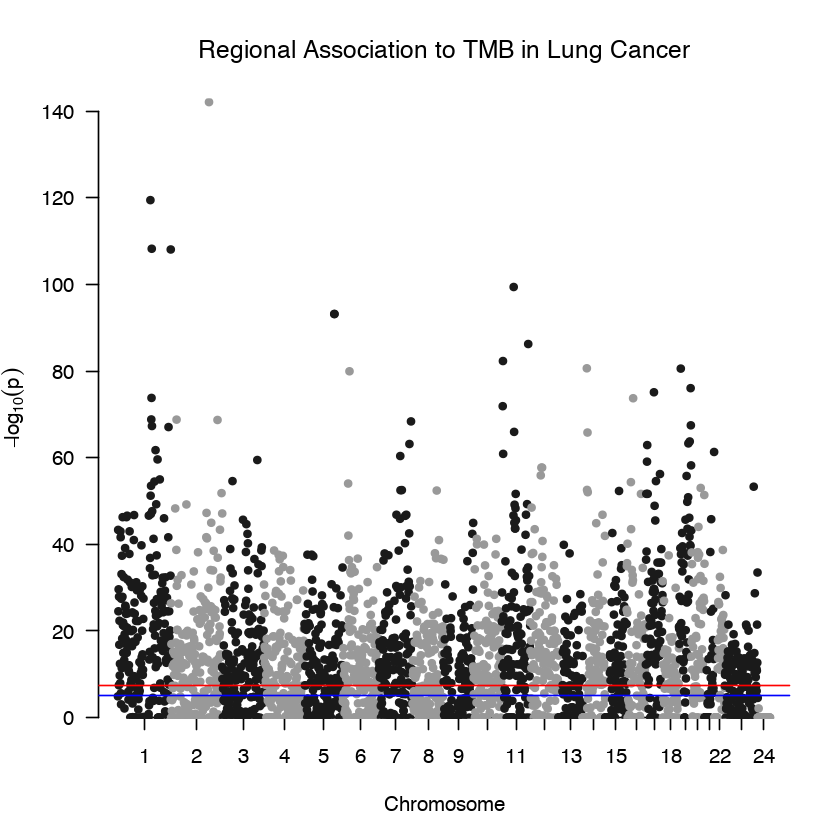
\includegraphics[width=5in]{figures/chapter1/lungmanhat.png}
\caption{For an additive, genome-wide biomarker such as TMB (Tumour Mutational Burden), all genomic loci are significantly correlated with TMB (unlike in typical GWAS studies). How do we choose a subset that isn't prohibitively large but can reliably estimate the marker via some predictive model? \label{fig:lungmanhat}}
\end{figure}

Suppose we have some set $G$ of genes, where $g$ refers to an individual gene with coding sequence of length $n_g$. Now let $P \subset G$ refer to a gene panel comprising a set of genes, and $\mathcal{M}_P$ be a model trained on some data with covariates included according to the gene panel $P$. Then we might wish to solve the optimisation problem 
\begin{equation}
\min_{P \subset G} \{\mathcal{L}(\mathcal{M}_P) \} \ \text{such that} \ |P| \leq L,
\end{equation} 
where $\mathcal{L}(\mathcal{M})$ is the loss of the model $\mathcal{M}$, $|P| = \sum\limits_{g \in P}n_g$ is the total length of the gene panel $P$ and $L$ is some prescribed maximum panel length. Note the similarity with the LASSO setup described in Section~\ref{sec:lasso}. In the case of a linear model we can similarly reformulate the problem in terms of the parameter $\mathbf{\beta}$, and solve the analogous problem. \\ ~ \\

\hrule
\begin{technique}{\textbf{(Weighted L1 Regularisation/LASSO)}} 
Here we select $\beta$ satisfying the optimisation problem
$$\min_{\beta \in \mathbb{R}^{|G|}} \{\mathcal{L(M}_\mathbf{\beta}) + \lambda\sum\limits_{g \in G}n_g|\beta_g| \} $$
where we have again swapped the panel length bound $L$ for the regularisation parameter $\lambda$. Since all the $n_g$ values are positive, this is still a convex optimisation problem and thus can be solved efficiency as in the standard case. Choice of $\lambda$ is less likely to be chosen via cross-fitting, as smaller values of $\lambda$ will always improve predictive power. Instead $\lambda$ will be chosen to control the size of the resulting gene panel.

\end{technique}
\hrule
~\\~\\

\subsubsection{Distinguishing causative mutations}
It should again be noted that these are illustrations of how high-dimensional model construction is done. In reality many more subtleties may have to be taken into account. In the above a key caveat requiring understanding is the role of selective pressure in cancer-relevant genes \citep{bull_unlocking_2013}, and how this affects the mutation rate in different sections of the genome \citep{iengar_identifying_2018}. One way this can be investigated is by looking at the relative predictive power of synonymous and non-synonymous mutations for genome-wide mutation burden \citep{chu_nonsynonymous_2019}. The gold standard for identifying causative relationships between genotype and phenotype, however, remains with functional validation studies.

\subsection{Survival prediction \label{sec:intro_survival}}
No review of statistical learning in cancer genomics would be complete without a mention of survival prediction. Survival prediction is useful in a variety of situations, far beyond direct prognostic application. Hazard regression models based on genomic data have been useful in identifying therapeutic resistance \citep{seagle_discovery_2016} or general prognosis \citep{guinney_prediction_2017, zhang_lassobased_2018} factors, which are of great interest to those developing drugs or attempting to understand which patients can expect to benefit from them. Regularisation based techniques are perfectly adaptable to proportional-hazards style models \citep{benner_high-dimensional_2010}, to which end there has much literature beyond what we have scope to discuss in this chapter. 

\section{Modern techniques in high-dimensional statistics and dimensionality reduction}
\epigraph{``c. 1950: Modern mathematics starts to take off. After that it gets complicated.''}{Professor Stewart's Hoard of Mathematical Treasures (\citeyear{stewart_professor_2010})}

We conclude with some examples from recent literature of techniques related to dimensionality reduction in modelling genomic data. The examples have been chosen to  demonstrate the structure/regularisation workflow discussed in this chapter, and are small a set of examples rather than (anywhere near) an exhaustive list.

\subsection{Regularised graphical models}
In the regression examples discussed previously, the parameters of interest have represented the weighted effect of observed covariates on a label. In supervised and unsupervised cases, we are also often interesting in looking at how closely related different covariates are, through estimating the correlation matrix of the observation variable $X$. If we have an observation of dimensionality $p$, then the covariance matrix will be of size $p^2$, so problems of estimation from small $n$ are even more confounded! 

Two forms of regularisation are popular, often used in tandem. The first is a sparsity penalty applied to all matrix entries \citep{witten_covariance-regularized_2009}. What does this correspond to structurally? It means that that most pairs of covariates are independent (or at least uncorrelated). This is a very relevant notion in network analysis, where variables are thought to affect each other in a way that can be described by some graphical structure. Sparsity of matrix elements then corresponds to sparsity of the graph describing the network. It is also not uncommon to sparsely penalise precision, defined by the components of the inverse covariance matrix \citep{xia_positive-definite_2017}. 

Alternately (or in addition), we may wish to limit the number of distinct \textit{patterns} of correlation, so that all covariates display a correlation profile that is made up of a combination of a relatively small set of base signatures. This structure may be fitted for by imposing rank-based regularisation \citep{ye_low-rank_2013, hu_low_2021}. For those wanting a greater appreciation of the theory, the way this is imposed is another good example of convex penalty relaxation (as was achieved by switching from the $L_0$ to $L_1$ norm in sparsity regularisation), where here the nuclear norm is used as the convex relaxation of matrix rank.  


\subsection{Localised sparsity assumptions}
We've made an extensive discussion of sparse models in this chapter. We might wonder if there are any generalisations to the assumption that relatively few of our covariates are important throughout all of our samples. One such generalisation would be that for some subsets of our samples sparsity assumptions hold, but that the important covariates may differ from subset to subset within our data. In a localised sparsity setting, we are often given some knowledge of the organisational structure of data, either in a discrete way through a prior partition of the samples or network structure, or in a continuous way through a measure of distance between samples (which may come directly from the input data). We can then fit linear models which are regularised towards sparsity, but where variable selection is allowed to vary between samples, and allowed to vary more between samples that are more distant. This has been applied to the prediction of drug toxicity based on differential gene expression data \citep{yamada_localized_2017}. 

\subsection{Variational autoencoders}
For our final example we consider a notion of dimensionality reduction which is more general and which has been studied extensively in the machine learning literature. This nicely elucidates the grey border between statistical and machine learning, and the difficulties and opportunities available to biological research by embracing the latter. 

Variational autoencoders (VAEs) are a class of neural networks with a variety of architectures and sizes, but whose premise centres around producing an encoding/decoding framework between high dimensional data and a lower dimensional representation \citep{kingma_auto-encoding_2022}. VAEs have an 'hourglass' shape: input data is fed into the network, and information is propagated through layers of progressively smaller size until a bottleneck is reached. The central layer will have some small number of latent nodes. Subsequent layers increase in size, reaching an output of dimension matching the input. VAEs are trained to reproduce the inputs with which they are trained as accurately as possible. We can then view the central latent nodes as an encoding of our input data \citep{zheng_understanding_2019}. This might \textit{a}) contain some insightful information, and \textit{b}) be useful as lower dimensional input data for training other models. 

In the context of cancer genomics \citep{way_extracting_2018}, VAEs pose two challenges, illustrative of those that machine learning procedures in general must overcome to be useful in a basic research or clinical setting. Firstly, they are highly parameterised compared to the types of model discussed so far. We've discussed at length the balance between data availability and model size, and the significant extra effort necessary to extract information when information is scarce. One of the advantages of deep learning procedures is their versatility and lack of dependence on prior knowledge and assumptions of structure. The cost is that they are very data intensive, prohibitively so in some cases. Secondly, while a VAE's latent nodes may be informative within a network, there is no necessary guarantee that they will be interpretable by a human, nor that biologically relevant features will have been neatly allocated to a single node. Strategies to 'untangle' VAEs are necessary to make biologically relevant predictions \citep{kompa_learning_2020}. 


\section{Conclusions}
The dimensionality of data in genomics is a sticking point that at its full potency is more debilitating than in any other research discipline \citep{barbour_precision_2019}. Even at the current pace of increase of the availability of sequencing data, it will be a long time away (if ever) that the most powerful and general machine learning techniques will be at our disposal without recourse to the vast wealth of biological knowledge we as a species have accumulated. To properly use that knowledge, we need researchers who are able to speak the language of both camps. It is not sufficient that researchers in cancer genomics provide data and questions to researchers in machine learning, nor that machine learning researchers communicate back the output of their methods. Instead, methods need to be crafted bespokely by those who understand what features of cancer data are relevant, how those features manifest themselves, and how to exploit them in a mathematically consistent way. 

This entire workflow is quite easy to follow when the sort of structure we are insisting upon in our models is very simple. Even when a structural assumption can be motivated in a single sentence (see Definition \ref{def:sparse}), and a model is simple (such as in linear regression), a good design of learning procedure might not be immediately obvious. It can likely, however, be given a fairly ground-up description within a single book chapter. When the structural assumptions we really want to incorporate might well extend as far as our current appreciation of the mutational processes affecting tumours across heterogenuous cell populations, chromosomes, genes and codons, and the models we want to fit are similarly at the cutting edge of computational research, then the position of an interdisciplinary researcher may well require far more legwork to maintain. 

As motivation for the above legwork, it should go without saying that cancer genomics in the machine learning age has potential to do a great deal of good in the long term. Yet uncovering a deeper understanding of how cancer works isn't the only worthwhile goal. Designing procedures that can work \textit{now} to be more effective, sometimes crossing a threshold between non-pracitcality and practicality (in some part of the world), can have a more immediate benefit. In the clinic, the time scale and cost of data collection aren't abstract mathematical problems, so designing a test that works with less data can be just as enabling as uncovering a new paradigm of cancer progression. 

\dobib % renders bibliography (only when compiling for chapter)


\end{document}